\documentclass[aspectratio=169]{beamer}
\usetheme{Madrid}
\usecolortheme{beaver}
\usepackage[utf8]{inputenc}
\usepackage[T1]{fontenc}
\usepackage{tikz}
\usepackage{amssymb}
\usepackage{graphicx}
\setbeamertemplate{navigation symbols}{}
\setbeamercolor{title}{fg=white,bg=cyan!60!black}
\setbeamercolor{frametitle}{fg=white,bg=cyan!50!black}
\setbeamercolor{block title}{bg=cyan!15,fg=black}
\setbeamercolor{block body}{bg=cyan!5,fg=black}

\title{G4 — My Blocks}
\subtitle{jump(), shoot(), spawnEnemy() — powers you define}
\author{ByteForge --- Grade 7 --- Game Maker --- Week Overview}
\date{}

\begin{document}

\begin{frame}
    \titlepage
\end{frame}

\begin{frame}{This Week's Plan}
    \begin{itemize}
        \item Lesson 1: spawnEnemy()
        \item Lesson 2: shoot()
        \item Lesson 3: powerUp()
        \item[$\bigstar$] BOSS --- Platformer Vertical Slice (\texttt{lessonBoss.tex})
    \end{itemize}
\end{frame}

\begin{frame}{Real-World Example}
    \Large
    A recipe you cook many times (make pancakes) is a "function" — the same steps, but the exact ingredients (parameters) change each time depending on how many people you're feeding. Minecraft's own crafting recipes are functions too: the SAME recipe (function) run with different wood types (the parameter) gives an oak vs. a birch door.
\end{frame}


\begin{frame}{Image}
    \begin{center}
    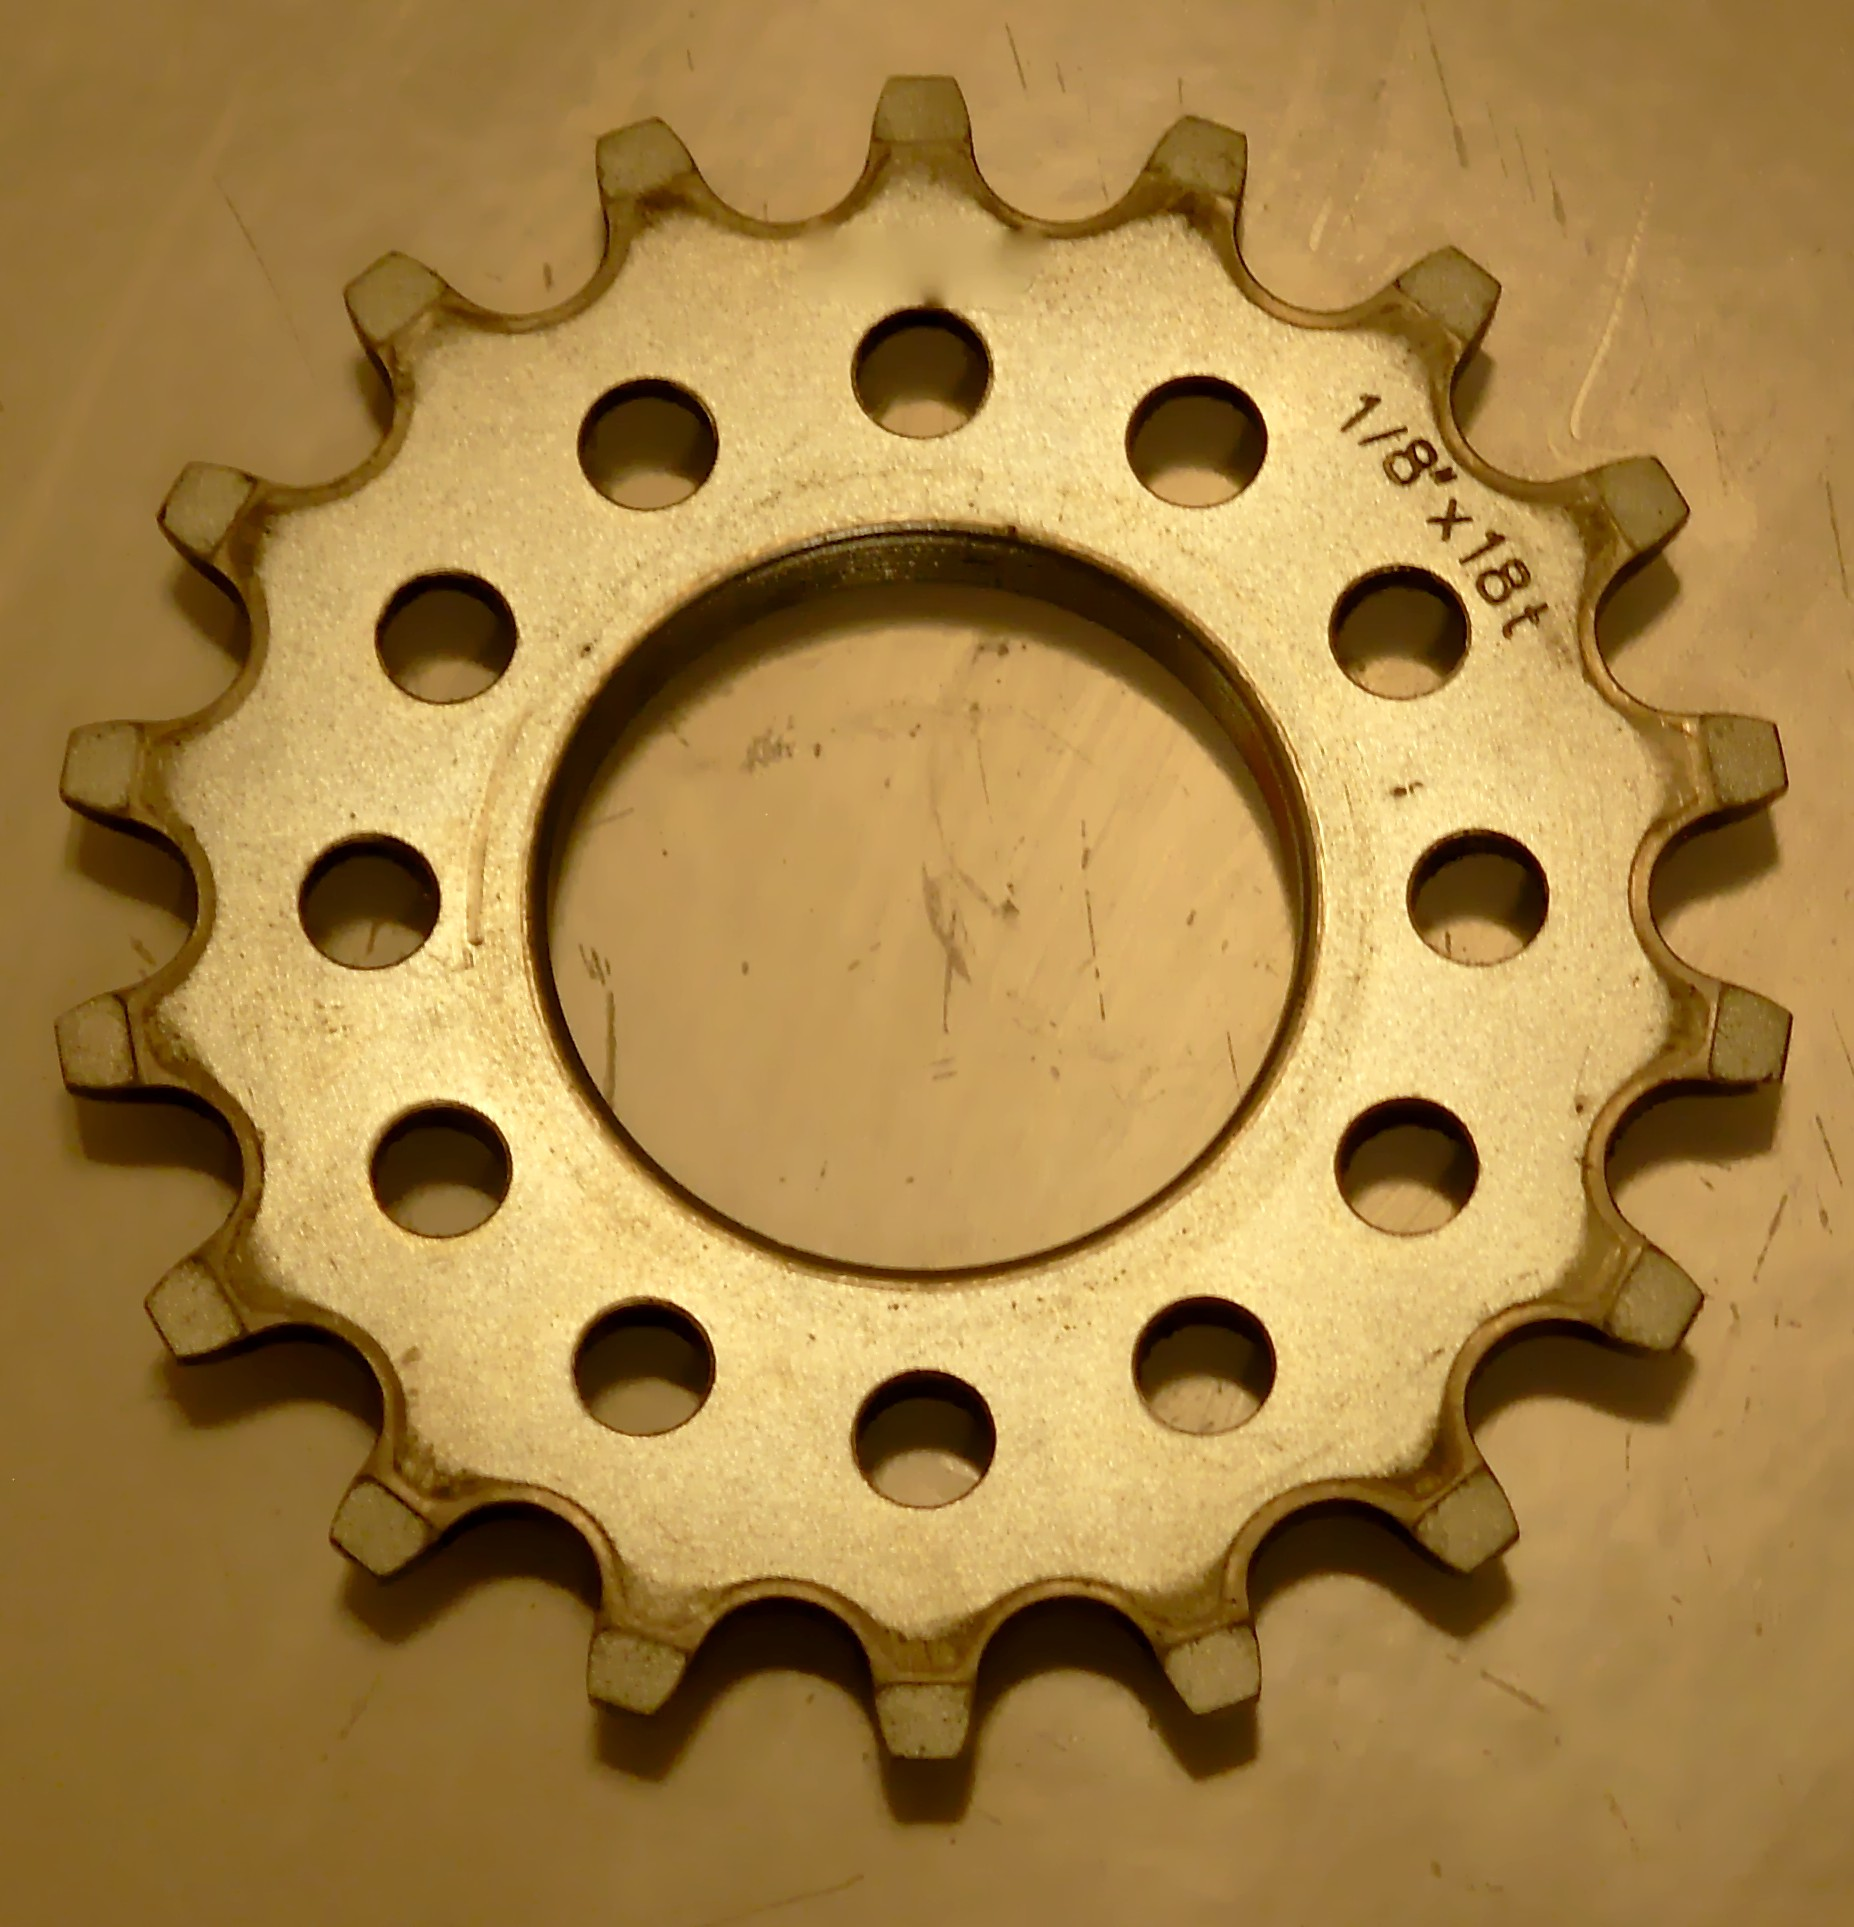
\includegraphics[width=0.55\textwidth]{../images/gear.jpg}

    \small Fixed gear cog — John Reaves, public domain, via Wikimedia Commons
    \end{center}
\end{frame}

\begin{frame}{Let Them Discover (1/2)}
    \Large
    Think of something you do repeatedly with small variations (making a sandwich, getting ready for school). Write the general steps once, then note which parts change each time (the "parameters").
\end{frame}


\begin{frame}{Let Them Discover (2/2)}
    \Large
    Pick any Minecraft recipe that works with more than one material (a door, a boat, tools). What stays exactly the same across every version, and what's the "parameter" that changes?
\end{frame}

\begin{frame}{Files in This Folder}
    \small
    \begin{itemize}
        \item \texttt{lesson1.tex} --- spawnEnemy()
        \item \texttt{lesson2.tex} --- shoot()
        \item \texttt{lesson3.tex} --- powerUp()
        \item \texttt{lessonBoss.tex} --- BOSS: Platformer Vertical Slice
    \end{itemize}
    \vspace{0.5em}
    \normalsize Each lesson file is its own short deck --- open the one for
    the specific day you're teaching, not this whole overview.
\end{frame}

\end{document}
